% Contribution chapter no. 5 (TOP20 pick 5, id ED-17) -- English translation of chapters/c05.tex
% Sources: papers/prog_superfluid_structure_factor/ (main.tex, AUDIT.md, REVISION.md, publication_meta.json,
% gen_numbers.tex, data/he4_Sk_donnelly_table14_1.csv, data/test_he4.csv), TOP20.json.
\chapter[A straight ruler, a wrong sketch]{A ruler proved straight shows that our own sketch was wrong}
\reference{Published on 26 October 2026.\\ doi:10.5281/\\zenodo.23653846}

\section*{The idea in one picture}

\begin{analogie}
You first prove that your ruler is perfectly straight. Then you lay it on a drawing you made yourself a few weeks
earlier, and you see that the drawing is crooked. The ruler is not at fault; the sketch is.

\emph{Where the picture stops:} here, the proved ``ruler'' speaks about an idealised model of a fluid; it is the
measurement of real helium, not the proof, that condemns the sketch.
\end{analogie}

\section*{What was done}

At very low temperature, liquid helium~4 becomes superfluid. It is studied by sending neutrons or X-rays into it and
measuring how they are deflected; from this one obtains the \emph{structure factor} $S(Q)$, which tells how the atoms
are organised at the scale $1/Q$. A classical argument links this measurement to the energy of the small waves that
travel through the fluid: at wave number $k$, the lowest energy is at most $\hbar^2k^2/(2mS(k))$, where $m$ is the
mass of one atom.

The work does two things. First, it writes and proves in Lean the mathematical core of this argument, explicitly
taking as assumptions two physical ingredients (a sum rule and a symmetry $k\leftrightarrow-k$) which are not
themselves proved in Lean. Second, it tests on published data an ``envelope'' that the project had proposed earlier
in the month, based on the idealised Bogoliubov gas model: $S(Q)\le B(Q)=\sqrt{Q/2k_*}$, with $k_*=2mc/\hbar$ and
$c=238.3$\,m/s the speed of sound in helium, which gives $k_*\approx3.004$\,Å$^{-1}$.

\begin{encadre}
\textbf{To do with a calculator: the top of the curve.} At the highest point of the table, $Q=2.058$\,Å$^{-1}$ and the
measured value is $S=1.458$. The envelope is $B=\sqrt{2.058/6.008}=\sqrt{0.3426}\approx0.585$. The measurement is
$1.458/0.585\approx2.49$ times higher than the proposed limit, and exceeds it by $0.87$, far more than the tolerance
margin of $0.082$.

\textbf{The idealised model itself respects the envelope.} In the Bogoliubov gas, $S=k/\sqrt{k_*^2+k^2}$. For
$k=k_*$, we get $1/\sqrt2\approx0.707$, and the envelope is $\sqrt{1/2}\approx0.707$: exact equality, never an
overshoot. This is the control case that must pass, and it does.
\end{encadre}

Of the 99 points of the reference table (X-ray and neutron measurements gathered in a published compilation), 29
respect the envelope, 7 exceed it by less than the margin (undecided) and 63 clearly exceed it (refuted). In the
so-called ``roton'' region, between $1.7$ and $2.4$\,Å$^{-1}$, all 21 points are refuted, by a factor of $1.62$ to
$2.49$ (figure~\ref{fig:c05}). The reading is modest: liquid helium is not a Bogoliubov gas, which textbooks already
say. The same paper therefore contains a positive formal result and a negative physical result, the latter about a
proposal of the project itself.

\begin{figure}[htbp]
\centering
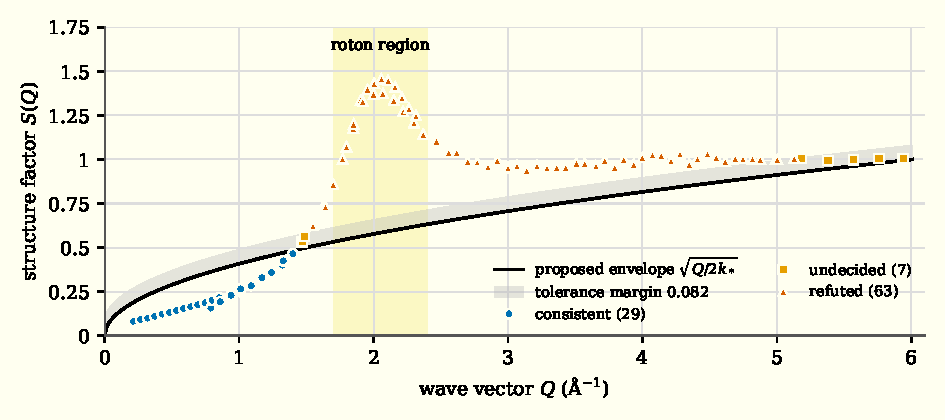
\includegraphics[width=\linewidth]{figures/c05_helium}
\caption{Tabulated structure factor of helium~4 (99 points) against the proposed envelope; verdicts recomputed with
the rule of the paper.}
\label{fig:c05}
\end{figure}

\section*{How we made sure it is not wrong}

\niveau{A} \emph{The judge looked}, for the mathematical part. Lean, the program that checks every step of a proof,
uses only the three basic assumptions accepted everywhere, and the module was replayed without error by a second
checking program on 26 October 2026. Two examples built on purpose show that the assumptions are not decorative: in
one, without the symmetry, the step that divides by two becomes false ($1$ instead of $1/2$); in the other, all the
assumptions hold at once and the bound is attained exactly. An independent AI agent recompiled everything on its own
side and slipped in two sabotages: an erased proof in an intermediate lemma was duly flagged, along with the three
main theorems that rely on it; a hidden axiom that ``proved'' an absurdity was also spotted.

The data are \niveau{L}: a published table, but second-hand, measured between 1.4 and 4 kelvins and without error
bars. The verdicts are \niveau{X}. The auditor re-read the raw table itself and found the same 29, 7 and 63. One
point is stated honestly: the margin of $0.082$ (the gap between the peaks of two series of measurements) was fixed
\emph{after} seeing the data, which departs from the announced plan. The roton result does not depend on it: its
smallest margin, $0.328$, is about four times this threshold, and it also holds on the subset of measurements that the
compilation itself recommends. This work was produced and audited by AI agents; no human specialist has reviewed it.

\section*{What this does not say}

\begin{limite}
\begin{itemize}
\item No novelty in physics is claimed: the argument is classical, and so is its conclusion about helium.
\item The physics of the argument (sum rule, symmetry) enters Lean as an assumption, not as a theorem.
\item The measurements are not at absolute zero, and the counts beyond $2.4$\,Å$^{-1}$ depend on the margin.
\item For gases of trapped atoms, the only values available were read off figures: no decisive test.
\end{itemize}
\end{limite}

\section*{Going further}

The paper shows that a solid proof and an honest measurement can together bring down a home-grown idea, and that this
retreat is published as progress. Paper: doi:10.5281/zenodo.23653846.
